\section{Methodology}

\blindtext[1]

\begin{table}[H]
    \caption{A Harmless Table}
    \begin{tabularx}{\linewidth}{>{\centering}X>{\centering}X>{\centering\arraybackslash}X}
        \toprule
        \textbf{Header} & \textbf{Header} & \textbf{Header}\\
        \midrule
        content & content & content \\
        content & content & content \\
        content & content & content \\
        \bottomrule
    \end{tabularx}
\end{table}

\blindtext[2]

\begin{figure}[H]
    \centering
    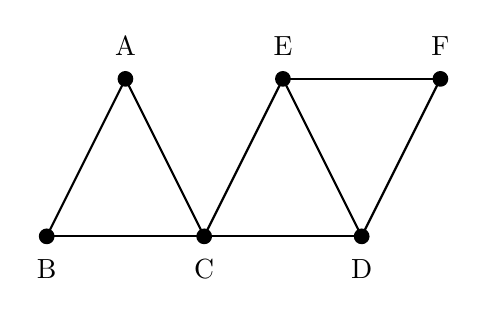
\begin{tikzpicture}[]
        \draw[thick] (0,0) -- (1,2);
        \draw[thick] (0,0) -- (2,0);
        \draw[thick] (1,2) -- (2,0);
        \draw[thick] (2,0) -- (3,2);
        \draw[thick] (3,2) -- (4,0);
        \draw[thick] (2,0) -- (4,0);
        \draw[thick] (3,2) -- (5,2);
        \draw[thick] (4,0) -- (5,2);
        \fill (0,0) circle (0.1) node[anchor=north, outer sep=5]{B};
        \fill (1,2) circle (0.1) node[anchor=south, outer sep=5]{A};
        \fill (2,0) circle (0.1) node[anchor=north, outer sep=5]{C};
        \fill (3,2) circle (0.1) node[anchor=south, outer sep=5]{E};
        \fill (4,0) circle (0.1) node[anchor=north, outer sep=5]{D};
        \fill (5,2) circle (0.1) node[anchor=south, outer sep=5]{F};
    \end{tikzpicture}
    \caption{Main Problem Graph}
\end{figure}

\begin{figure}[H]
    \centering
    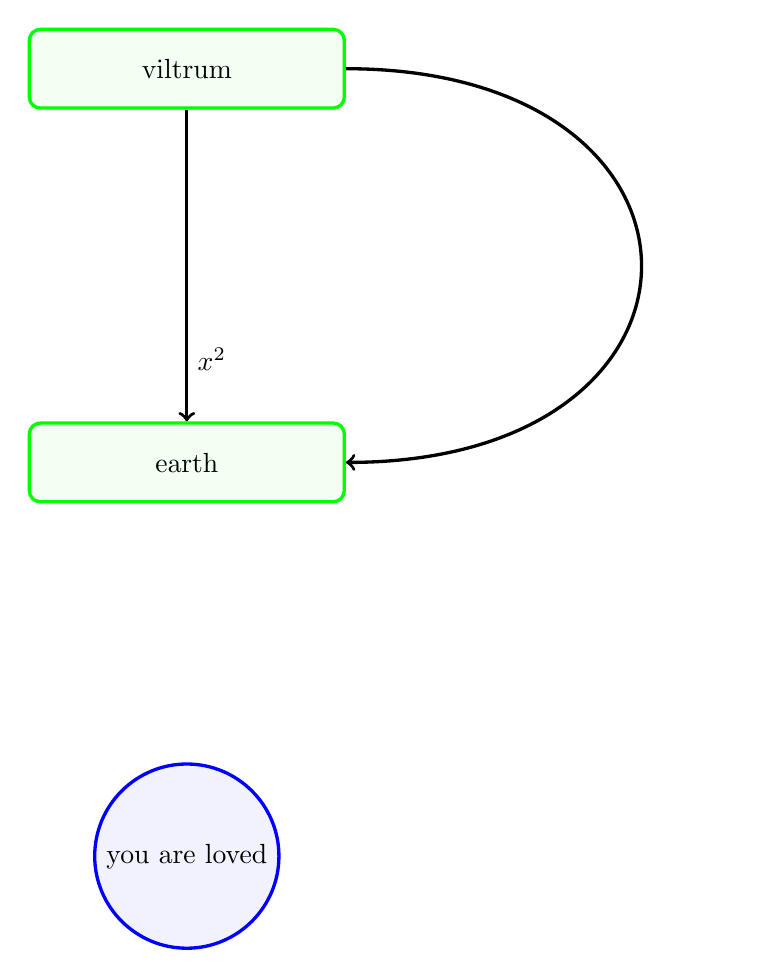
\begin{tikzpicture}[
            no/.style={
                rectangle,
                draw=green,
                fill=green!5,
                very thick,
                rounded corners,
                minimum width=4cm,
                minimum height=1cm,
                text centered
            },
            ci/.style={
                circle,
                draw=blue,
                fill=blue!5,
                very thick,
                minimum size=1.5cm,
                text centered
            }
            % transform canvas={scale=1.0}
        ]

        % nodes
        \node[no] (n1) at (0, 0) {viltrum};
        \node[ci] (main) at (0, -10) {you are loved};
        \node[no] (n2) at (0, -5) {earth};

        % lines
        \draw[->, very thick] (n1.south) to node[right, pos=0.8] {$x^2$} (n2.north);
        \draw[->, very thick] (n1.east) .. controls +(right:5cm) and +(right:5cm) .. (n2.east);
    \end{tikzpicture}
\end{figure}

\blindtext[2]
